% Created 2024-02-22 Thu 10:55
% Intended LaTeX compiler: pdflatex
\documentclass[presentation]{beamer}
\usepackage[utf8]{inputenc}
\usepackage[T1]{fontenc}
\usepackage{graphicx}
\usepackage{longtable}
\usepackage{wrapfig}
\usepackage{rotating}
\usepackage[normalem]{ulem}
\usepackage{amsmath}
\usepackage{amssymb}
\usepackage{capt-of}
\usepackage{hyperref}
\mode<beamer>{\usetheme{Madrid}}
\definecolor{SUred}{rgb}{0.59375, 0, 0.17969} % SU red (primary)
\definecolor{SUblue}{rgb}{0, 0.17578, 0.38281} % SU blue (secondary)
\setbeamercolor{palette primary}{bg=SUred,fg=white}
\setbeamercolor{palette secondary}{bg=SUblue,fg=white}
\setbeamercolor{palette tertiary}{bg=SUblue,fg=white}
\setbeamercolor{palette quaternary}{bg=SUblue,fg=white}
\setbeamercolor{structure}{fg=SUblue} % itemize, enumerate, etc
\setbeamercolor{section in toc}{fg=SUblue} % TOC sections
% Override palette coloring with secondary
\setbeamercolor{subsection in head/foot}{bg=SUblue,fg=white}
\setbeamercolor{date in head/foot}{bg=SUblue,fg=white}
\institute[SU]{Shenandoah University}
\titlegraphic{
\includegraphics[width=0.5\textwidth]{\string~/Documents/suLogo/suLogo.pdf}}
\newcommand{\R}{\mathbb{R}}
\usepackage{tikz}
\usepackage{pgfplots}
\usetheme{default}
\author{Chase Mathison\thanks{cmathiso@su.edu}}
\date{26 February 2024}
\title{Other Trigonometric Integrals}
\hypersetup{
 pdfauthor={Chase Mathison},
 pdftitle={Other Trigonometric Integrals},
 pdfkeywords={},
 pdfsubject={},
 pdfcreator={Emacs 29.1 (Org mode 9.6.7)}, 
 pdflang={English}}
\begin{document}

\maketitle

\section{Announcements}
\label{sec:orgcda46e5}
\begin{frame}[label={sec:orge9acb5b}]{Announcements}
\begin{enumerate}
\item Exam corrections due Tuesday.
\item Homework in MyOpenMath (One due Wednesday, one due next Monday)
\end{enumerate}
\end{frame}

\section{Lecture}
\label{sec:orga2c53e4}
\begin{frame}[label={sec:org76c169d}]{Tangent and secant}
Instead of showing you all of the cases that we can encounter
involving \(\tan(x)\) and \(\sec(x)\), let's jump to the general
strategy, because the process is largely the same as before:
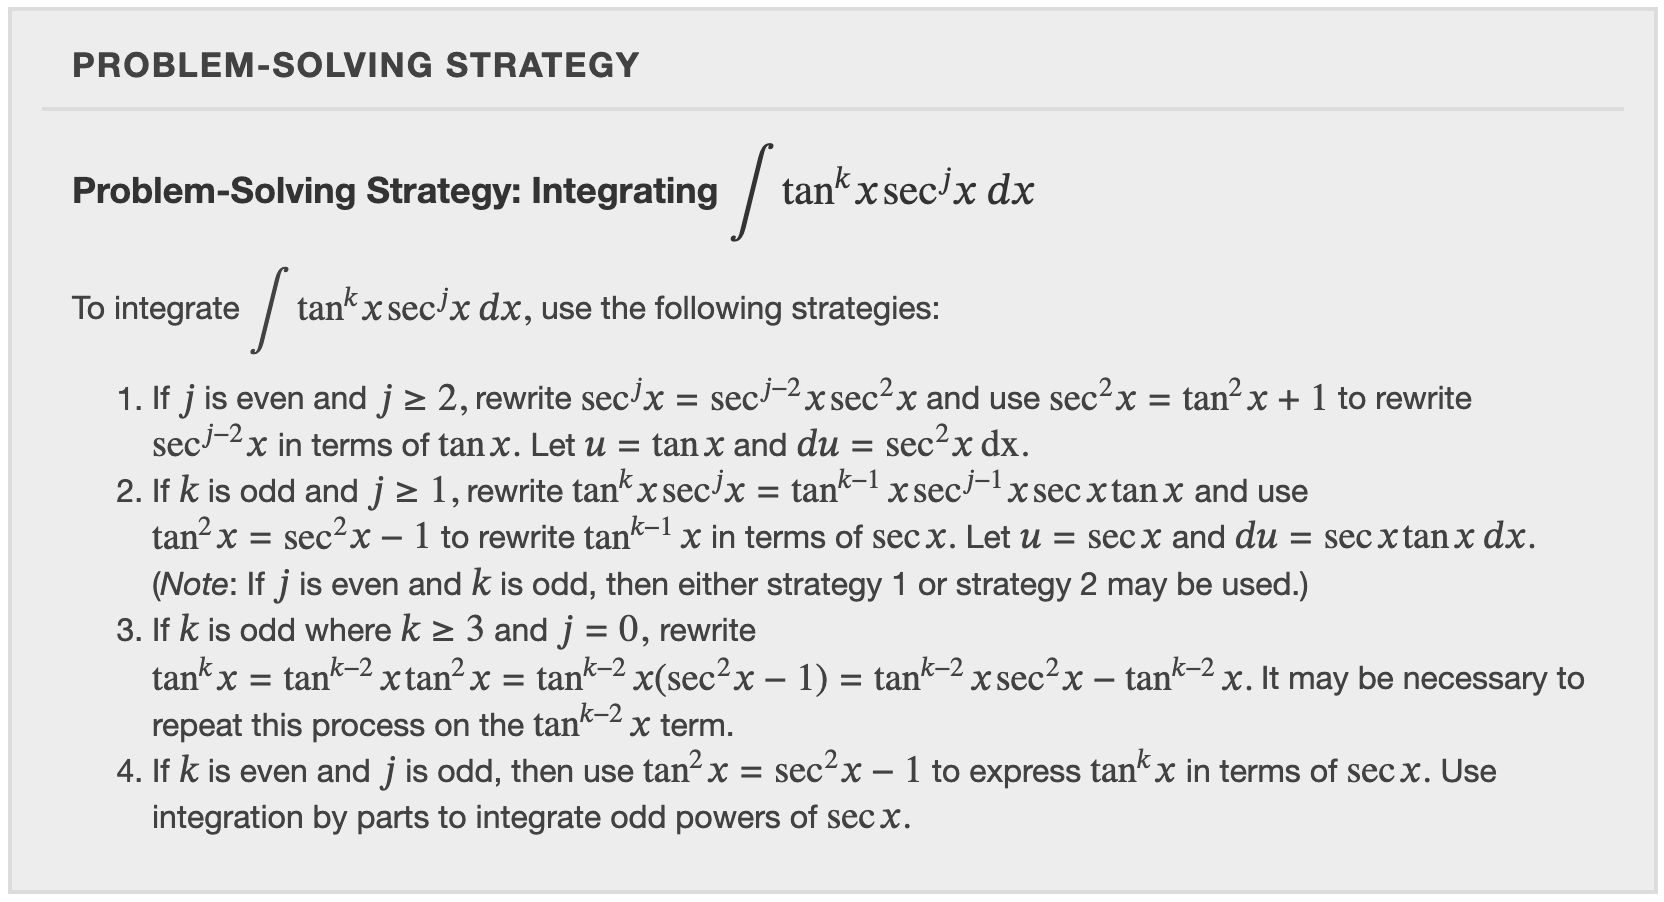
\includegraphics[width=\textwidth]{../img/day018-03.png}
\end{frame}

\begin{frame}[label={sec:org13c4a91}]{A few special cases}
Here are a few special cases that don't quite follow those rules:
\begin{enumerate}
\item \(\int\limits_{}^{} \sec^2 x\,dx =\)
\item \(\int\limits_{}^{} \sec(x)\tan(x)\,dx =\)
\item \(\int\limits_{}^{} \tan(x)\,dx =\)
\item \(\int\limits_{}^{} \sec(x)\,dx =\)
\end{enumerate}
\end{frame}

\begin{frame}[label={sec:orgabb6146}]{Example}
Evaluate
\[
\int\limits_{}^{} \sec^4(x)\tan(x)\,dx \]
\vspace{10in}
\end{frame}

\begin{frame}[label={sec:org5e3202f}]{Example}
\end{frame}

\begin{frame}[label={sec:org74b18d6}]{Example}
Evaluate
\[
\int\limits_{}^{} \tan^5(x)\sec(x)\,dx \]
\vspace{10in}
\end{frame}

\begin{frame}[label={sec:org5881662}]{Example}
\end{frame}

\begin{frame}[label={sec:org106f301}]{Example}
Evaluate
\[
\int\limits_{}^{} \tan^3 (x)\,dx \]
\vspace{10in}
\end{frame}

\begin{frame}[label={sec:org05177c7}]{Example}
\end{frame}

\begin{frame}[label={sec:orgbc39f8a}]{Power Reduction Formula}
Let's develop a power reduction formula for \(\int\limits_{}^{} \sec^n(x)\,dx\) if \(n\ge 3\) is odd. (This will really help us with the next example).
\[
I_n = \int\limits_{}^{} \sec^n(x)\,dx\]
\vspace{10in}
\end{frame}

\begin{frame}[label={sec:org9740fa9}]{Example}
\end{frame}

\begin{frame}[label={sec:orge3023bd}]{Example}
Evaluate
\[
\int\limits_{}^{} \tan^4(x)\sec(x)\,dx\]
\vspace{10in}
\end{frame}

\begin{frame}[label={sec:orge04f28e}]{Example}
\end{frame}
\end{document}